\loesung{

\textbf{Prerequisites:}

We will need a few general facts about least-squares linear regression for this exercise:

\begin{enumerate}[1.]

\item 
The formulae for estimating the parameters $\hat{\beta}_0$ and $\hat{\beta}_1$ of the linear regression model.
These formulae can be calculated from the model equation $\hat{f}_{LM} (x) = \hat{y} = \hat{\beta}_0 + \hat{\beta}_1 x$ and the loss equation $SSE_{LM} = \sum_{i=1}^n \left( y^{(i)} - \hat{f}_{LM}(x^{(i)}) \right)^2$ using standard calculus.

\begin{gather*}
\hat{\beta}_0 = \bar{y} - \hat{\beta}_1 \bar{x}
\, \ \Longleftrightarrow \, \
\bar{y} = \hat{\beta}_0 + \hat{\beta}_1 \bar{x}
\\
\hat{\beta}_1 = \frac{ \sum_{i=1}^n (x^{(i)} - \bar{x})(y^{(i)} - \bar{y}) }{\sum_{i=1}^n (x^{(i)} - \bar{x})^2}  
\end{gather*}

One can prove (with standard multivariate calculus) that these values of the parameters are the unique minimizers of the loss function.
It follows that:

$$
(\hat{y}^{(i)} - \bar{y}) = \hat{\beta}_0 + \hat{\beta}_1 x^{(i)}- (\hat{\beta}_0 + \hat{\beta}_1 \bar{x}) = \hat{\beta}_1 (\hat{x}^{(i)} - \bar{x}).
$$

\item
With the notation

\begin{align*}
    SSE_{LM} &= \sum_{i=1}^n (y^{(i)} - \hat{f}_{LM}(x^{(i)}))^2 = \sum_{i=1}^n (y^{(i)} - \hat{y}^{(i)})^2 &\text{ for the sum of squared errors (the loss) from the regression,} \\
	SSE_{c} &= \sum_{i=1}^n (y^{(i)} - \bar{y})^2 &\text{ for the total sum of squares / the variance of the data points,}\\
	SSE_{LM-c} &= \sum_{i=1}^n (\hat{y}^{(i)} - \bar{y})^2 = \sum_{i=1}^n (\hat{f}_{LM}(x^{(i)}) - \bar{y})^2 &\text{ for the total sum of squares / the variance of the predictions,}
\end{align*}

the following holds:

\begin{equation}\label{eq:lin_model_pythagoras}
    SSE_{c} = SSE_{LM} + SSE_{LM-c} \
    \ \ \Longleftrightarrow \ \ \
    \sum_{i=1}^n (y^{(i)} - \bar{y})^2
    = \sum_{i=1}^n (y^{(i)} - \hat{y}^{(i)})^2
    + \sum_{i=1}^n (\hat{y}^{(i)} - \bar{y})^2
\end{equation}

This basically means that the model predictions \(\hat{y}_i\) and the residuals \( (y_i - \hat{y}_i) \) are uncorrelated.
(The two vectors are "orthogonal" to each other.)
A proof for formula \eqref{eq:lin_model_pythagoras} is given below.

\item
We can use \eqref{eq:lin_model_pythagoras} to rewrite the coefficient of determination as follows:

\begin{align*}
    R^2 = 1-\frac{SSE_{LM}}{SSE_{c}} = \frac{SSE_{LM-c}}{SSE_{c}} = \frac{\sum_{i=1}^n (\hat{y}^{(i)} - \bar{y})^2}{\sum_{i=1}^n (y^{(i)} - \bar{y})^2}
\end{align*}

%Recall that the formula for the coefficient of determination $R^2$ is:
%\begin{align*}
%	R^2 = 1-\frac{SSE_{LM}}{SSE_{c}} = 1 - \frac{\sum_{i=1}^n (y^{(i)} - \hat{f}_{LM}(x^{(i)}))^2}{\sum_{i=1}^n (y^{(i)} - \bar{y})^2}
%	= 1 - \frac{\sum_{i=1}^n (y^{(i)} - \hat{y}^{(i)})^2}{\sum_{i=1}^n (y^{(i)} - \bar{y})^2}
%\end{align*}
%where $SSE_{LM} = \sum_{i=1}^n (y^{(i)} - \hat{f}_{LM}(x^{(i)}))^2$ is the sum of squares due to regression (error) and $SSE_{c} = \sum_{i=1}^n (y^{(i)} - \bar{y})^2$ is the total sum of squares. 

An illustration of this relation:

\begin{center}
	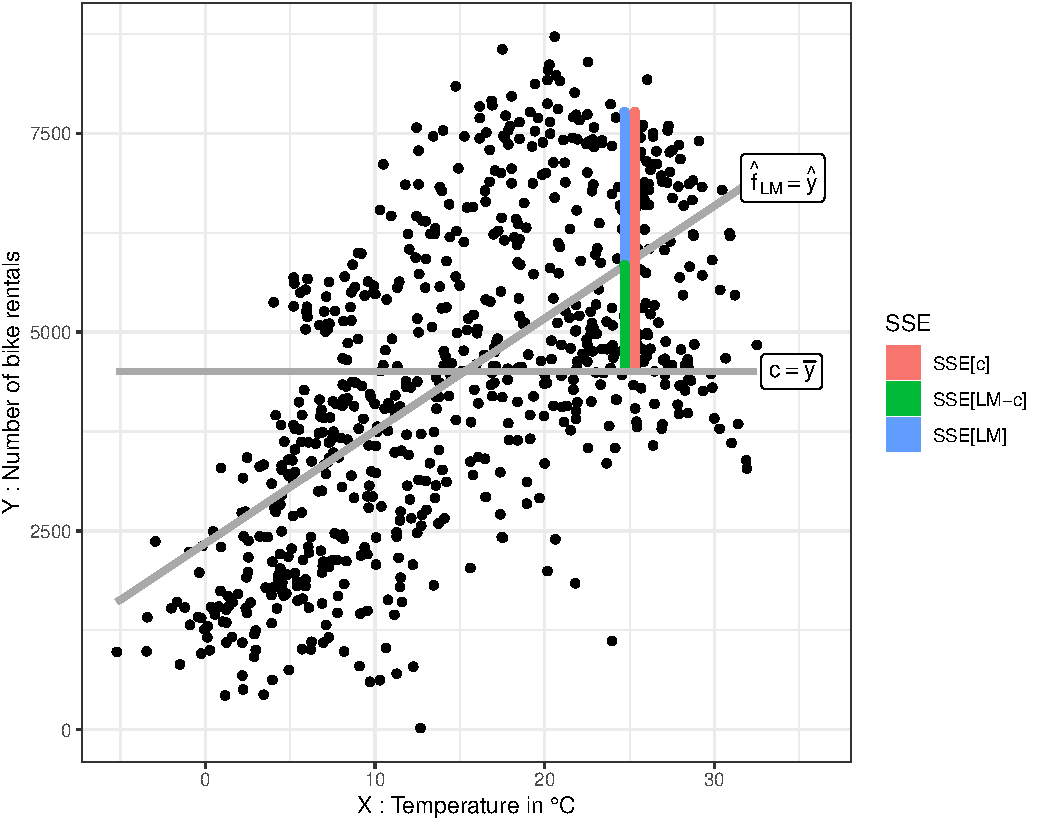
\includegraphics[width=0.75\maxwidth]{figure/r_squared.pdf}
\end{center}

\end{enumerate}

%First it is shown that 
%\begin{align} \label{P2}
%	R^2 = 1-\frac{SSE_{LM}}{SSE_{c}} = 1 - \frac{\sum_{i=1}^n (y^{(i)} - \hat{y}^{(i)})^2}{\sum_{i=1}^n (y^{(i)} - \bar{y})^2}
%	= \frac{\sum_{i=1}^n (\hat{y}^{(i)} - \bar{y})^2}{\sum_{i=1}^n (y^{(i)} - \bar{y})^2} = \frac{SSE_{LM-c}}{SSE_{c}}
%\end{align}

\textbf{Proof of equation \eqref{eq:lin_model_pythagoras}:}

\fbox{\parbox{\linewidth}{
		
We want to show:

%\begin{align} %\label{P1}
$$
	\sum_{i=1}^n (y^{(i)}-\bar{y})^2 = \sum_{i=1}^n (y^{(i)}-\hat{y}^{(i)})^2 + \sum_{i=1}^n (\hat{y}^{(i)} - \bar{y})^2.
$$
%\end{align}
%Proof: 

Because of

\begin{align*}
	\sum_{i=1}^n (y^{(i)}-\bar{y})^2 
	&= \sum_{i=1}^n (y^{(i)} - \hat{y}^{(i)} + \hat{y}^{(i)} - \bar{y})^2 \\
	&= \sum_{i=1}^n (y^{(i)} - \hat{y}^{(i)})^2 + (\hat{y}^{(i)} - \bar{y})^2 + 2(y^{(i)}-\hat{y}^{(i)})(\hat{y}^{(i)} - \bar{y}) \\
	&= \sum_{i=1}^n (y^{(i)} - \hat{y}^{(i)})^2 + \sum_{i=1}^n(\hat{y}^{(i)} - \bar{y})^2 + 2\sum_{i=1}^n(y^{(i)}-\hat{y}^{(i)})(\hat{y}^{(i)} - \bar{y}),
\end{align*}

%It remains to show that 
it is sufficient to show that the following covariance vanishes:

$$
\sum_{i=1}^n (y^{(i)}-\hat{y}^{(i)}) (\hat{y}^{(i)} - \bar{y}) = 0
$$

This is indeed the sample covariance between \( (y^{(i)}-\hat{y}^{(i)}) \) and \( \hat{y}^{(i)} \) (or equivalently between \( (y^{(i)}-\hat{y}^{(i)}) \) and \( (\hat{y}^{(i)} - \bar{y}) \)), because $ \bar{\hat{y}} = \frac{1}{n} \sum_{i=1}^n \hat{y}^{(i)} = \bar{y} $ is the average of \(\hat{y}^{(i)}\) and therefore $ (y^{(i)}-\hat{y}^{(i)}) $ has an average of 0.

}}

\fbox{\parbox{\linewidth}{

%\begin{align*}
%	\sum_{i=1}^n(y^{(i)}-\hat{y}^{(i)})(\hat{y}^{(i)} - \bar{y}) &= 0 \\
%	\sum_{i=1}^n (y^{(i)}-\hat{y}^{(i)})\hat{y}^{(i)} - \sum_{i=1}^n (y^{(i)}-\hat{y}^{(i)})\bar{y}&= 0 \\
%	\bar{y}\, \sum_{i=1}^n y^{(i)}-\hat{y}^{(i)} &= 0 \\
%	\sum_{i=1}^n y^{(i)}-\hat{y}^{(i)} &= 0
%\end{align*}

%where we have used the fact that $\sum_{i=1}^n (y^{(i)}-\hat{y}^{(i)})\hat{y}^{(i)} = 0$ as the residuals $(y^{(i)}-\hat{y}^{(i)})$ and $\hat{y}^{(i)}$ are not correlated. 

We start with the formula for \(\hat{\beta}_1\):

\begin{align*}
    & & \hat{\beta}_1 &= \frac{ \sum_{i=1}^n (x^{(i)} - \bar{x})(y^{(i)} - \bar{y}) }{\sum_{i=1}^n (x^{(i)} - \bar{x})^2} \\
    & \Rightarrow & \hat{\beta}_1 \sum_{i=1}^n (x^{(i)} - \bar{x})^2 &= \sum_{i=1}^n (x^{(i)} - \bar{x})(y^{(i)} - \bar{y}) \\
    & \Leftrightarrow & 0 &= \sum_{i=1}^n (x^{(i)} - \bar{x})(y^{(i)} - \bar{y}) - \hat{\beta}_1 \sum_{i=1}^n (x^{(i)} - \bar{x})^2 
    = \sum_{i=1}^n \left( (x^{(i)} - \bar{x})(y^{(i)} - \bar{y}) - \hat{\beta}_1 (x^{(i)} - \bar{x})^2 \right) \\
    & & &= \sum_{i=1}^n \left( (y^{(i)} - \bar{y}) - \hat{\beta}_1 (x^{(i)} - \bar{x}) \right) (x^{(i)} - \bar{x})
    = \sum_{i=1}^n \left( (y^{(i)} - \bar{y}) - (\hat{y}^{(i)} - \bar{y}) \right) (x^{(i)} - \bar{x}) \\
    & & &= \sum_{i=1}^n (y^{(i)} - \hat{y}^{(i)}) (x^{(i)} - \bar{x}) \\
    & \Rightarrow & 0 &= \hat{\beta}_1 \sum_{i=1}^n (y^{(i)} - \hat{y}^{(i)}) (x^{(i)} - \bar{x})
    = \sum_{i=1}^n (y^{(i)} - \hat{y}^{(i)}) (\hat{\beta}_1 (x^{(i)} - \bar{x}))\\
    & & &= \sum_{i=1}^n (y^{(i)} - \hat{y}^{(i)}) (\hat{y}^{(i)} - \bar{y})
\end{align*}
\hfill (proof of \eqref{eq:lin_model_pythagoras}) $\Box$ \\
}}

\bigskip

%It follows: 
%\begin{align*}
%	R^2 &=  1 - \frac{\sum_{i=1}^n (y^{(i)} - \hat{y}^{(i)})^2}{\sum_{i=1}^n (y^{(i)} - \bar{y})^2} 
%	= \frac{\sum_{i=1}^n (y^{(i)} - \bar{y})^2 - \sum_{i=1}^n (y^{(i)} - \hat{y}^{(i)})^2}{\sum_{i=1}^n (y^{(i)} - \bar{y})^2}\\
%	&= \frac{\sum_{i=1}^n (y^{(i)}-\hat{y}^{(i)})^2 + \sum_{i=1}^n (\hat{y}^{(i)} - \bar{y})^2 - \sum_{i=1}^n (y^{(i)} - \hat{y}^{(i)})^2}{\sum_{i=1}^n (y^{(i)} - \bar{y})^2}
%	= \frac{\sum_{i=1}^n (\hat{y}^{(i)} - \bar{y})^2}{\sum_{i=1}^n (y^{(i)} - \bar{y})^2}
%\end{align*}
%\hfill (proof of (\ref{P2})) $\Box$ \\ 

\textbf{Proof of \(R^2 = \rho^2\):}

%And further: 
We start with $R^2$ and plug in the functional equation from the regression for the data points and for the sample averages. A little more calculation yields the desired result:
\begin{align*}
	R^2
    &= \frac{\sum_{i=1}^n (\hat{y}^{(i)} - \bar{y})^2}{\sum_{i=1}^n (y^{(i)} - \bar{y})^2}
	%= \frac{\sum_{i=1}^n(\hat{\beta}_0 + \hat{\beta}_1 x^{(i)}- (\hat{\beta}_0 + \hat{\beta}_1 \bar{x}))^2}{\sum_{i=1}^n (y^{(i)} - \bar{y})^2}
	%= \frac{\hat{\beta}_1^2 \sum_{i=1}^n (x^{(i)} - \bar{x})^2}{\sum_{i=1}^n (y^{(i)} - \bar{y})^2}
    = \frac{ \sum_{i=1}^n (\hat{\beta}_1 (x^{(i)} - \bar{x}))^2}{\sum_{i=1}^n (y^{(i)} - \bar{y})^2}
    = \hat{\beta}_1^2 \, \frac{\sum_{i=1}^n (x^{(i)} - \bar{x})^2}{\sum_{i=1}^n (y^{(i)} - \bar{y})^2}  \\
    &= \left(\frac{\sum_{i=1}^n (x^{(i)} - \bar{x})(y^{(i)} - \bar{y})}{\sum_{i=1}^n (x^{(i)} - \bar{x})^2}\right)^2 \frac{\sum_{i=1}^n (x^{(i)} - \bar{x})^2}{\sum_{i=1}^n (y^{(i)} - \bar{y})^2} 
    = \frac{ \left( \sum_{i=1}^n (x^{(i)} - \bar{x})(y^{(i)} - \bar{y}) \right)^2 }{\sum_{i=1}^n (x^{(i)} - \bar{x})^2 \sum_{i=1}^n (x^{(i)} - \bar{x})^2} \frac{\sum_{i=1}^n (x^{(i)} - \bar{x})^2}{\sum_{i=1}^n (y^{(i)} - \bar{y})^2} \\
    &= \frac{\left(\sum_{i=1}^n (x^{(i)} - \bar{x})(y^{(i)} - \bar{y})\right)^2}{\sum_{i=1}^n (x^{(i)} - \bar{x})^2\sum_{i=1}^n (y^{(i)} - \bar{y})^2} \\
    &= \rho^2
\end{align*}

%Now, starting with $\rho^2$, we can write:
%\begin{align*}
% 	\rho^2 &= \left(\frac{\sum_{i=1}^n (x^{(i)} - \bar{x})(y^{(i)} - \bar{y})}{\sqrt{\sum_{i=1}^n (x^{(i)} - \bar{x})^2}\sqrt{\sum_{i=1}^n (y^{(i)} - \bar{y})^2}}\right)^2 \\
%	&= \frac{\left(\sum_{i=1}^n (x^{(i)} - \bar{x})(y^{(i)} - \bar{y})\right)^2}{\sum_{i=1}^n (x^{(i)} - \bar{x})^2\sum_{i=1}^n (y^{(i)} - \bar{y})^2}\\
%	&= \frac{\left(\sum_{i=1}^n (x^{(i)} - \bar{x})(y^{(i)} - \bar{y})\right)^2}{\sum_{i=1}^n (x^{(i)} - \bar{x})^2\sum_{i=1}^n (y^{(i)} - \bar{y})^2} \frac{\sum_{i=1}^n (x^{(i)} - \bar{x})^2}{\sum_{i=1}^n (x^{(i)} - \bar{x})^2}\\
%	&= \left(\frac{\sum_{i=1}^n (x^{(i)} - \bar{x})(y^{(i)} - \bar{y})}{\sum_{i=1}^n (x^{(i)} - \bar{x})^2}\right)^2 \frac{\sum_{i=1}^n (x^{(i)} - \bar{x})^2}{\sum_{i=1}^n (y^{(i)} - \bar{y})^2} \\
%	&= \hat{\beta}_1^2 \, \frac{\sum_{i=1}^n (x^{(i)} - \bar{x})^2}{\sum_{i=1}^n (y^{(i)} - \bar{y})^2}
%	= R^2
%\end{align*}

%$\Rightarrow R^2 = \rho^2$.
%
%\bigskip
%
%\textbf{Option 2:}
%\begin{align*}
%	R^2 &= 1 - \frac{SSE_{LM}}{SSE_{c}} = 1 - \frac{\sum_{i=1}^n (y^{(i)} - \hat{y}^{(i)})^2}{\sum_{i=1}^n (y^{(i)} - \bar{y})^2} \\
%	&= \frac{\sum_{i=1}^n (\hat{y}^{(i)} - \bar{y})^2}{\sum_{i=1}^n (y^{(i)} - \bar{y})^2} 
%\end{align*}

This shows $R^2 = \rho^2$, which completes the proof.
\hfill $\Box$ \\
\vspace*{-0.3cm}

Note that this result is only valid for simple linear regression, only for the case of one independent variable, and also only for regression with ordinary least squares (OLS). For multiple regression, the coefficient of determination is defined differently and does not necessarily equal the square of the Pearson correlation coefficient.

Similar proofs together with more information: \\
https://statproofbook.github.io/P/slr-rsq.html \\
https://math.stackexchange.com/questions/129909/correlation-coefficient-and-determination-coefficient

}
